\documentclass{article}
\usepackage{graphicx}

\title{Report Labwork 4}
\author{Ha Trung Hieu}


\begin{document}

\maketitle

\textbf{Threads}

\begin{itemize}
	\item Firstly, I calculate the size of pixels.
		
	\item Secondly, I allocate the input memory and the ouput memory of CUDA with \textit{cudaMalloc()} function.
	\item Thirdly, I copy CUDA Memory from CPU to GPU with \textit{cudaMemcpy()} function in \textit{cudaMemcpyHostToDevice} mode.
	\item Fourthly, I set the block size \textit{blockSize} to 64 and calculate number of block equal to \[blockSize = pixelCount / (blockSize * 3)\].
	\item Fifthly, I init the \textit{rgb2grayCUDA<<<numBlock, blockSize>>>()} with the input memory and the output memory.
	\item Sixthly, I copy the ouput image with \textit{cudaMemcpy()} function in \textit{cudaMemcpyDeviceToHost} mode.
	\item Finally, I clear the memory with \textit{cudaFree()} function.
	\item The result:\newline
	\begin{figure}[ht]
	\centering
	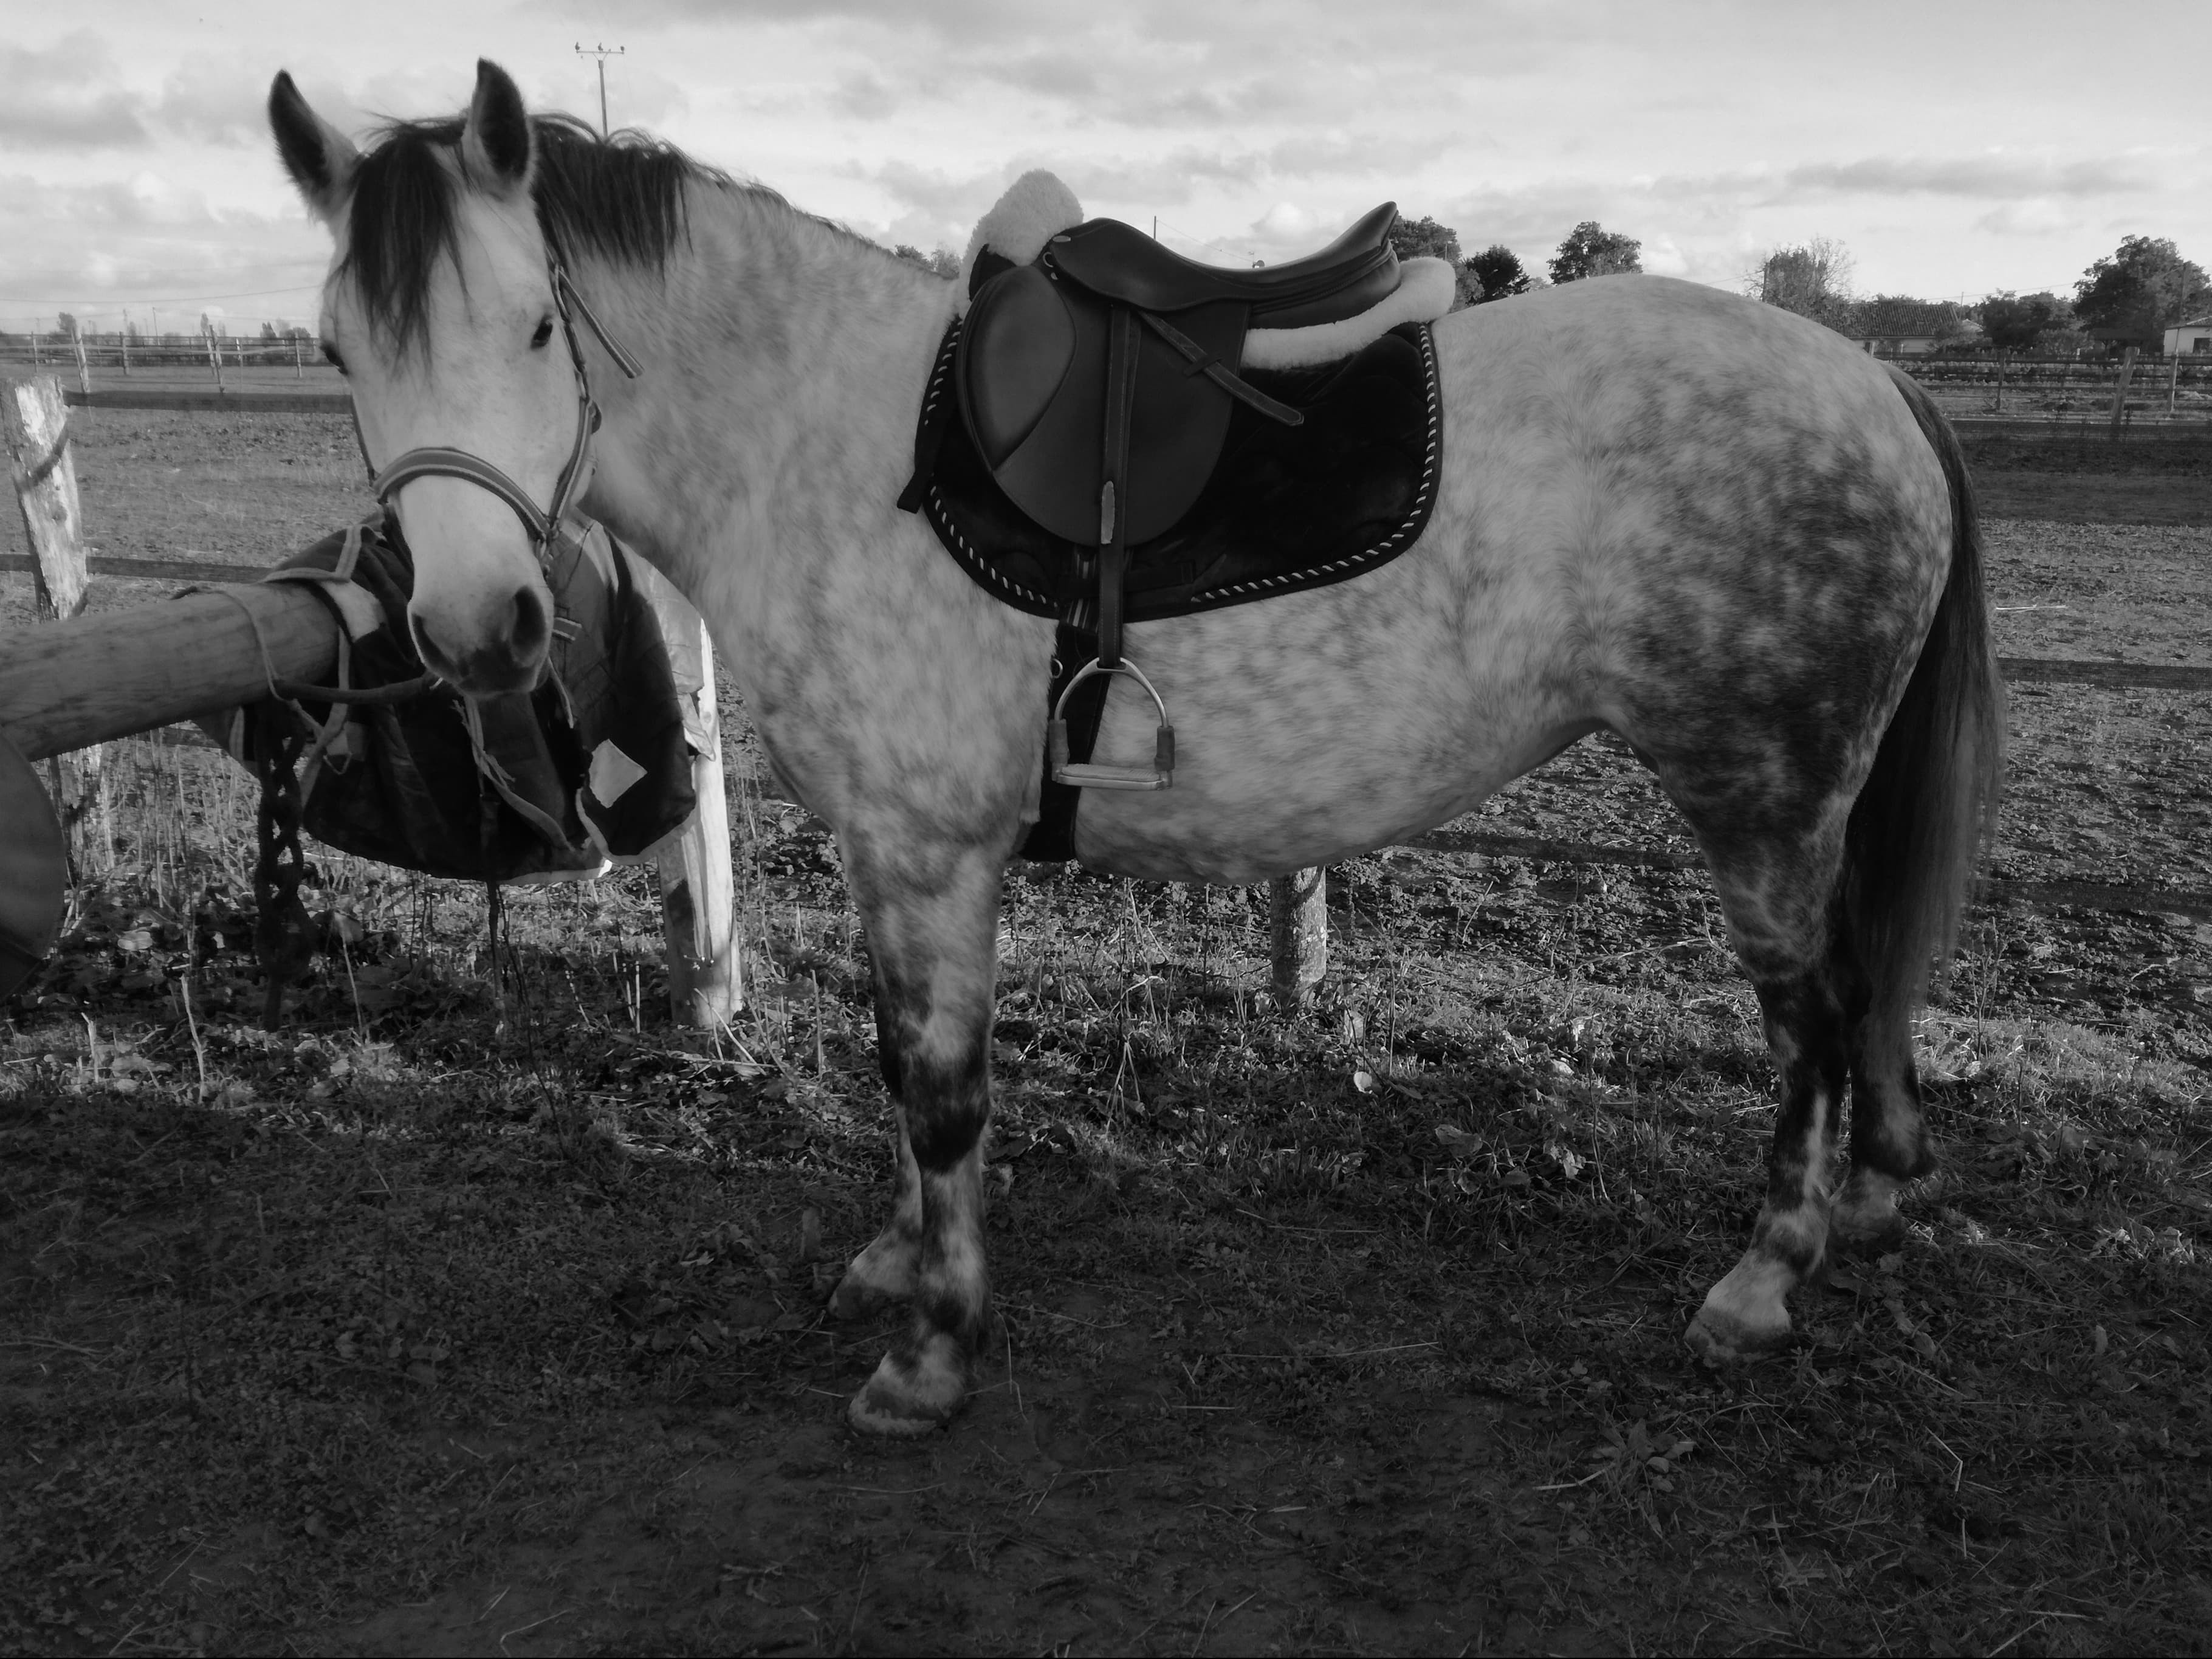
\includegraphics[width=.8\textwidth]{labwork4-gpu-out.jpg}
	\caption{Labwork output image}
	\label{fig:cat_laptop}
	\end{figure}
	
	USTH ICT Master 2018, Advanced Programming for HPC.\newline
    Warming up...\newline
    Starting labwork 3\newline
    labwork 3 ellapsed 10.7ms\newline
\end{itemize}
\end{document}